\documentclass[format=acmsmall, review=false]{acmart}


\usepackage{acm-ec-17}

\usepackage{booktabs} % For formal tables
\usepackage[ruled]{algorithm2e} % For algorithms
\graphicspath{ {experiments/} }
\usepackage{subcaption}

\renewcommand{\algorithmcfname}{ALGORITHM}
\SetAlFnt{\small}
\SetAlCapFnt{\small}
\SetAlCapNameFnt{\small}
\SetAlCapHSkip{0pt}
\IncMargin{-\parindent}

\usepackage{graphicx}     			% can better scale and rotate graphics than graphic package
\usepackage{multirow}               		% allows to have table cells on more than one row with "\multirow"
%\usepackage{amsmath, amsthm}	% !!! not for ACM template !!!
\usepackage{amssymb}                	% allows special symbols like "\nexists"
\usepackage{latexsym}               		% ? Dan
\usepackage{alltt}                  		% ? Dan
\usepackage{amsgen}                 	% ? Dan
\usepackage{amstext}               		% ? Dan
\usepackage{amscd}                  		% ? Dan
\usepackage{algorithmic}
\usepackage{url}
\usepackage{enumerate}
%\usepackage{cases}                  		% ? Dan
\usepackage{amsthm}
%\usepackage{mathtools}
%\usepackage{savesym}
\usepackage{amsmath}
\usepackage{tikz}
\usepackage{float}
\usepackage{enumitem}
\usepackage{mdwlist}
\usepackage{xspace}
\usetikzlibrary{arrows.meta}
%\savesymbol{iint}
%\usepackage{txfonts}
%\restoresymbol{TXF}{iint}
\usepackage{bm}                     	% bold Greek letters
\usepackage{upgreek}              
\usepackage{xspace}    
\usepackage{color}              
\usepackage{colortbl}    
\usepackage{tabularx}
\usepackage{aliascnt}  	
\usepackage{mdframed}
\usepackage{caption}
\usepackage{makecell}
\usepackage{tcolorbox}
\usepackage{float}                 % Should be included for hyperref according to Google Groups + algorithm + hyperref + float; in fact messes links to algorithms up


\newcommand{\shaleen}[1]{{\color{blue} Shaleen: [{#1}]}}
\newcommand{\paris}[1]{{\color{red} Paris: [{#1}]}}
\newcommand{\todo}[1]{{\color{red} ToDo: {#1}}}
\newcommand{\cull}[1]{{\color{red} [{#1}]}}
\newcommand{\introparagraph}[1]{\textbf{#1.}}   
\newcommand{\cut}[1]{}

\newenvironment{packed_item}{
\begin{itemize}
   \setlength{\itemsep}{1pt}
   \setlength{\parskip}{0pt}
   \setlength{\parsep}{0pt}
}
{\end{itemize}}

\newenvironment{packed_enum}{
\begin{enumerate}
   \setlength{\itemsep}{1pt}
  \setlength{\parskip}{0pt}
   \setlength{\parsep}{0pt}
}
{\end{enumerate}}

\newenvironment{packed_grep}{
\begin{description}
   \setlength{\itemsep}{1pt}
   \setlength{\parskip}{0pt}
   \setlength{\parsep}{0pt}
}
{\end{description}}
              
\newcommand{\ie}{{\em i.e.}\xspace}
\newcommand{\eg}{{\em e.g.}\xspace}
\newcommand{\ea}{{\em et al.}\xspace}
\newcommand{\aka}{{\em a.k.a.}\xspace}

\newcommand{\dtr}[0]{\twoheadrightarrow}     
 
\newcommand{\bQ}[0]{\mathbf{Q}}       
\newcommand{\bD}[0]{\mathbf{D}}       
\newcommand{\bR}[0]{\mathbf{R}}       
\newcommand{\bU}[0]{\mathbf{U}}     
\newcommand{\bT}[0]{\mathbf{T}}     
\newcommand{\bA}[0]{\mathbf{A}}     
\newcommand{\bB}[0]{\mathbf{B}}     
\newcommand{\bAp}[0]{\mathbf{A}}     
\newcommand{\bBp}[0]{\mathbf{B}}     
\newcommand{\bC}[0]{\mathbf{C}}     
\newcommand{\bV}[0]{\mathbf{V}}   
\newcommand{\bG}[0]{\mathbf{G}}     
 
\newcommand{\mS}[0]{\mathcal{S}} 
\newcommand{\mI}[0]{\mathcal{I}}   
\newcommand{\mF}[0]{\mathcal{F}}   
\newcommand{\mH}[0]{\mathcal{H}}   
\newcommand{\mE}[0]{\mathcal{E}}   
\newcommand{\mV}[0]{\mathcal{V}}   
\newcommand{\mC}[0]{\mathcal{C}}      
\newcommand{\mM}[0]{\mathcal{M}}   
\newcommand{\mL}[0]{\mathcal{L}}   
\newcommand{\mP}[0]{\mathcal{P}}   

\newcommand{\APS}[0]{\textsf{APS}}   
\newcommand{\DPS}[0]{\textsf{DPS}} 
\newcommand{\QPS}[0]{\textsf{QPS}} 

\newcommand{\agr}[2]{\mS_{#1}(#2)} 
\newcommand{\dagr}[2]{{\mC}_{#1}(#2)} 
\newcommand{\setof}[2]{\{{#1}\mid{#2}\}}
\newcommand{\set}[1]{\{#1\}}   
\newcommand{\qb}[1]{\langle {#1} \rangle}   

\newcommand{\cmark}{\ding{51}}%
\newcommand{\xmark}{\ding{55}}%
\newcommand{\db}{\mathcal{D}}%
\newcommand{\upd}{\textsf{up}^\uparrow}

\newcommand{\ubp}{\textsf{UBP}}
\newcommand{\uip}{\textsf{UIP}}
\newcommand{\lpip}{\textsf{LPIP}}
\newcommand{\cip}{\textsf{CIP}}

\newcommand{\ra}[1]{\renewcommand{\arraystretch}{#1}}

\definecolor{Gray}{gray}{0.9}
\definecolor{cardinal}{rgb}{0.77, 0.12, 0.23}
\definecolor{bondiblue}{rgb}{0.0, 0.58, 0.71}
\definecolor{babyblue}{rgb}{0.54, 0.81, 0.94}
\definecolor{lightgreen}{rgb}{0.67, 0.94, 0.82}
\definecolor{maize}{rgb}{0.98, 0.93, 0.37}

\hypersetup{colorlinks,citecolor={cardinal}}  

%\DeclareRobustCommand{\hlrone}[1]{{\sethlcolor{babyblue}\hl{#1}}}
%\DeclareRobustCommand{\hlrtwo}[1]{{\sethlcolor{maize}\hl{#1}}}
%\DeclareRobustCommand{\hlrthree}[1]{{\sethlcolor{lightgreen}\hl{#1}}}

\newcommand{\hlrone}[1]{{\color{black} {#1}}}
\newcommand{\hlrtwo}[1]{{\color{black} {#1}}}
\newcommand{\hlrthree}[1]{{\color{black} {#1}}}
\newcommand{\cmr}[1]{{\color{black} {#1}}}




\begin{document}
% Title portion. Note the short title for running heads 
\title[Revenue Maximizing Algorithms for Query Pricing]{Revenue Maximization for Query Pricing : Approximation Algorithms and Practical Advances}  



\begin{abstract}
In this paper, we present approximation algorithms for {\em query pricing} problem so as to maximize seller's revenue in the unlimited supply setting. We formulate the problem as an instance item pricing over {\em item hypergraph} where the buyers are {\em single minded} with subadditive valuations and investigate a variety of pricing strategies including {\em uniform item pricing} and {\em uniform bundle pricing}. \cite{guruswami2005profit} gave an $O(\log m + \log n)$ where $m$ is the number of customers and $n$ is the number of items with sum of all valuations as the upper bound. In our setting, we show that both item pricing and uniform bundle pricing exhibit a gap of $\Omega(m)$ from the optimal subadditive bundle pricing. Additionally, we investigate the revenue obtained using XOS pricing functions and show $O(\dots)$ approximation with a matching lower bound. We complement our theoretical results with extensive experiments on industry scale workloads. To this end, our experiments show that pricing algorithms behave very well in practice when valuations are drawn randomly from a variety of distributions including zipfian, normal and uniform distribution.
\end{abstract}


\maketitle

\section{Introduction}
\label{sec:intro}

The last decade or so has seen an explosion of data being collected from a variety of sources and across a broad range of areas. Many companies, including Bloomberg~\cite{bloomberg}, Twitter~\cite{twitterapi}, Lattice Data~\cite{lattice}, DataFinder~\cite{datafinder}, and Banjo~\cite{banjo} collect such data, which then sell as structured (relational) datasets. 
These datasets are also often sold through online {\em data markets}, which are web platforms for buying and selling data: examples include BDEX~\cite{bdex}, Salesforce~\cite{salesforce} and QLik DataMarket~\cite{qlik}. Even though data sellers and data markets offer an abundance of data products, the pricing schemes currently used are very simplistic. In most cases, a data buyer has only one option, to buy the whole dataset (or a bundle of datasets) at a fixed price. Alternatively, the dataset is split into multiple disjoint chunks, and each chunk is sold at a separate price. 

However, data buyers are commonly interested in extracting specific information from a dataset, and not in acquiring the whole dataset. Accessing this information can be often concisely captured through a {\em query}, or a sequence of queries. Selling the whole dataset to a fixed price forces the buyer to either pay for the query more than it is valued, or to choose to not access it. This means that valuable data is often not accessible to lay users, scientists, or entities with limited budgets, and moreover that data-selling companies and marketplaces behave suboptimally with respect to maximizing their revenue.

To address this problem, a recent line of research~\cite{KUBHS12,KUBHS13,deep2017qirana} in the database community introduced the framework of  query-based pricing. A {\em query-based pricing scheme} tailors the purchase of the data to the user's needs, by assigning a price to each query issued over the dataset. Given a dataset $\db$ and a query $Q$ over the dataset, the user must pay a price $p(Q,\db)$ to obtain the answer $Q(\db)$ of the query. This price reflects only the value of the information learned by obtaining the query answer, and not the computational cost of executing the query. The work on query-based pricing has mainly focused on how one can define a well-behaved pricing function, and to how to compute it efficiently. In particular, a key property that a pricing function must obey is that of {\em arbitrage freeness}: it should not be possible for the buyer to acquire a query for a cheaper price through the combination of other query results. The arbitrage-free constraint makes the design of appropriate pricing functions a challenging task, especially since deciding whether a query is more informative than another query (or set of queries) is generally a computationally hard problem, and for practical applications it is critical that the price computation can be performed efficiently.

To overcome this computational barrier, one possible solution proposed in~\cite{deep2017qirana}  is to model each query $Q$ as a {\em bundle} of items $B(Q)$ from a common itemset $I$. Then, the arbitrage-free constraint translates to the requirement that the pricing function must be {\em monotone} and {\em subadditive} when viewed as a set function. Among such set functions, of particular practical interest are the additive and constant functions. An additive function gives to each item $i \in I$  a weight $w_i \geq 0$, and assigns the price $p(Q,\db) = \sum_{i \in B(Q)} w_i$, while a constant function simply assigns the same  price to every query, \ie $p(Q,\db) = p$.
However, prior work has not answered the fundamental question of how one can choose among the possible set functions (or subclasses of them) the one that maximizes the revenue of the seller. 

In this paper, we tackle the above question building on ideas from the optimal pricing 
literature~\cite{guruswami2005profit}. We consider the {\em unlimited supply} setting, where the 
seller can sell any number of units of each query. This is a natural assumption in the context of a data market,
since multiple buyers can request and purchase the same query.
Additionally, we assume that the buyers are {\em single-minded}, so each
buyer is interested in buying only a single query $Q$ (so a single bundle) for a price of $v_Q$; the buyer will
purchase the query only if the price $p(Q, \db)$ does not exceed $v_Q$. We focus on the aforementioned two
types of pricing functions that either assign a uniform price to every query, or perform item pricing. 
In the case of item pricing, the problem of computing the revenue-maximizing prices can be cast as
the well-studied {\em hypergraph vertex pricing} problem, where only approximation guarantees are known.



\paragraph{Our Contribution.}








\section{Related Work}
\label{sec:related}

Here goes related work.

1. Query-based pricing.

2. Item pricing: algorithms and lower bounds.



%
\section{Notation and Preliminaries}

We assume that there are $m$ customers (hyperedges) and $n$ items. Since we are in the {\em unlimited supply setting}, the seller has zero marginal cost  for each item, i.e, the seller can sell any number of units of each item. Additionally, the buyers are  {\em single minded}, which means that each customer is interested in buying only a single set of items corresponding to the hyperedge $e$ for price $v_e$. Buyers will purchase $e$ only if the price assigned to bundle $e$ is atmost $v_e$. We will use $p^{b}_e$ and $p^{i}_e$ to denote the bundle and item prices respectively assigned by the algorithm. 
\section{The Query-Based Pricing Framework}
\label{sec:framework}


\textbf{\textit{Question 1.}} Given $m$ customers (hyperedges) and their valuations $v_i$, what is the revenue gap between the optimal arbitrage free pricing and: $(i)$ item pricing $(ii)$ uniform bundle pricing, using the pricing function $p^{a}(Q,\mathcal{D})$.

\vspace{1em}
We show that the gap is $\Omega(m)$ for uniform bundle pricing and this is tight. For item pricing, we show that gap is $\Omega(m)$. Given these results, it is tantalizing to wonder whether XOS pricing functions (rather than single additive function) helps bridge the revenue gap. 

\vspace{1em}
\textbf{\textit{Question 2.}} Given $m$ customers (hyperedges) and their valuations $v_i$, what is the revenue gap between the optimal arbitrage free pricing and XOS pricing function.

\vspace{1em}
Our main result for the second question is 

\section{Uniform Bundle and Item Pricing}

In this section, we show our results for uniform bundle and item pricing. Figure~\ref{fig:summary} summarizes the main results. 


\begin{figure}[t]
	\scalebox{.95}{
		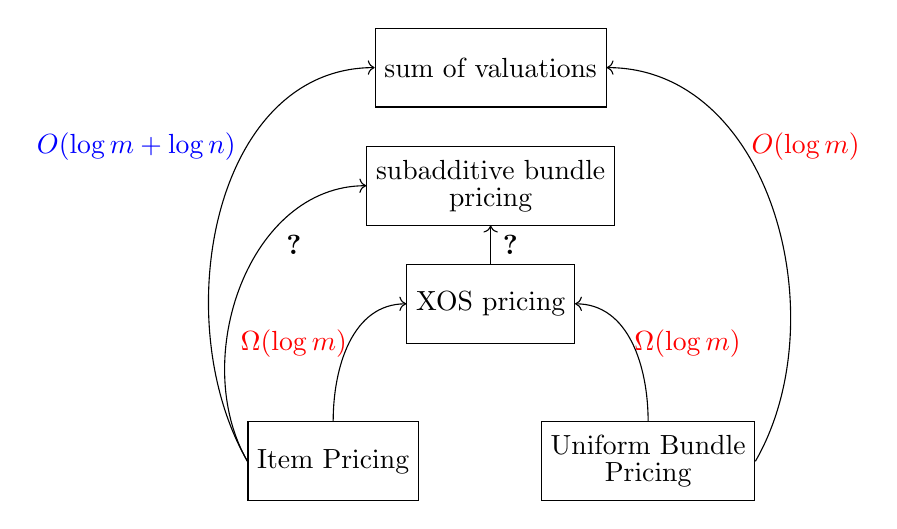
\begin{tikzpicture}
		\node (rectsum) [rectangle, draw, minimum width=7mm, minimum height=10mm] at (0,1.5) {sum of valuations};
		
		\node (rectbundle) [rectangle, draw, minimum width=7mm, minimum height=10mm] at (0,0) {\shortstack{subadditive bundle \\ pricing}};
		
		\node (rectxos) [rectangle, draw, minimum width=7mm, minimum height=10mm] at (0,-1.5) {XOS pricing};
		
		\node (rectitem) [rectangle, draw, minimum width=7mm, minimum height=10mm] at (-2,-3.5) {Item Pricing};
		
		\node (rectubundle) [rectangle, draw, minimum width=7mm, minimum height=10mm] at (2,-3.5) {\shortstack{Uniform Bundle \\ Pricing}};
		
		\draw [->] (rectubundle.east) to [out=60, in = 0] (rectsum);
		\node at (4,0.5) {\textcolor{red}{$O( \log m)$}};
		\draw [->] (rectubundle) to [out=90, in = 0] (rectxos);
		\node at (2.5,-2) {\textcolor{red}{$\Omega( \log m)$}};
		\draw [->] (rectitem.west) to [out=120, in = -180] (rectsum.west);
		\node at (-4.5,0.5) {\textcolor{blue}{$O( \log m + \log n)$}};
		\draw [->] (rectitem) to [out=90, in = -180] (rectxos.west);
		\node at (-2.5,-2) {\textcolor{red}{$\Omega( \log m)$}};
		\draw [->] (rectxos) to  (rectbundle);
		\node at (0.25,-0.75) {\textbf{?}};
		\draw [->] (rectitem.west) [out = 120, in = -180] to  (rectbundle.west);
		\node at (-2.5,-0.75) {\textbf{?}};
		
		\end{tikzpicture}
	}
	\caption{Results Summary: Red font show results in this paper; blue font shows existing known results}
	\label{fig:summary}
\end{figure}

\subsection{Uniform Bundle Pricing}

We begin by proving the $O(\log m)$ upper bound with respect to sum of valuations. 

\begin{lemma}
	Consider a hypergraph $\mH = (\mV, \mE)$ with $m$ edges and valuation $v_e$ for each edge $e \in \mE$. Then, there exists a uniform price $p'$ such that $p^{b}_e = p'$ achieves $O(\log m)$-approximation. 
\end{lemma}
\begin{proof}
	Consider the valuations $v_{e_1}, v_{e_2}, \dots, v_{e_m}$ in increasing order. We claim that $ p^{b}_e  = v_{e_{i'}}$ achieves the desired approximation for some edge $e_{i'}$. Assume for the sake of contradiction that this is not the case. Let $\textsf{OPT} = \sum_{e \in \mE} v_e$. Then $m v_{e_1} < \textsf{OPT}/ \log m$ since we can sell each edge if the bundle price is the smallest valuation. Similarly, $(m - i) v_{e_i} < \textsf{OPT}/ \log m$ for each edge. Adding up all inequalities, we get:
	
	\begin{equation}
	\begin{aligned}
	\textsf{OPT} = \sum_{e \in \mE} v_e & < \frac{\textsf{OPT}}{\log m} (\frac{1}{m} + \frac{1}{m-1} + \dots + 1) \\
	& \leq \textsf{OPT}
	\end{aligned}
	\end{equation}
	
	which is a contradiction.
\end{proof}

Next, we show that the $O(\log m)$ upper bound is tight.

\begin{lemma}
	There exists a set of buyers with XOS valuations such that any uniform bundle price produces revenue atmost $\textsf{OPT}/ \log m$.
\end{lemma}	
\begin{proof}
	Consider $n=m$ items and $m$ buyers such that buyer $b_i$ wants item $i$ for price $1/i$. It is easy to see that the valuations are XOS and achieves a revenue of $\log m$. Consider any fixed $p^b_e = 1/c$ such that $1 \leq c \leq m$. Then, the seller can sell edges that have valuation atleast $1/c$. Observe that the number of such edges is atmost $c$. Therefore, the revenue is atmost $\sum_{e:v_e \leq 1/c} 1/c = O(1)$.
\end{proof}

\subsection{Item Pricing}

Next, we show the $\Omega(\log m)$ gap between item pricing and XOS pricing.

\begin{lemma}
	There exists a set of buyers with XOS valuations such no item pricing solution can obtain revenue better than $\textsf{OPT}/ \log m$.
\end{lemma}
\begin{proof}
	Let $\mC_i$ denote the class of customers that desire exactly $\vert i \vert$ items. We construct the hypergraph instance as follows: Each class of customers $\mC_i$ has exactly $\lceil n/i \rceil$ and each customer in $\mC_i$ is assigned a partition of $i$ items such that no two customers share any item. Thus, the total number of hyperedges is $m = \sum_{i} \vert \mC_i \vert = \Theta( n \log n)$. Figure shows  an instance for $n=6$. We fix the valuation $v_e = 1$ for all hyperedges. This set of valuations is XOS and the revenue obtained by selling each edge at price $p^{b}_e = 1$ extracts the full revenue of $\Theta(n \log n)$.
	
	Next, we show that no item pricing solution can do better than $O(n)$. We will show this by induction on the customer class $\mC_i$. The base case is revenue obtained by selling edges to customers in $\mC_1$. Since there are atmost $n$ edges, the maximum revenue is $O(n)$. Consider the customer class $\mC_k$. Let denote $0 < \alpha \leq 1$ be the fraction of edges sold to customers in $\mC_k$ and let $\mE_k$ denote such edges. Then, the maximum revenue that can be extracted is $\alpha \lceil n/k \rceil$. We distinguish three types of edges: $(i)$ edges that share atleast one item with edges in $\mE_k$ $(ii)$ edges that do not share any item with edges in $\mE_k$ $(iii)$ edges that are strictly contained within $\mE_k$. By the induction hypothesis, the maximum revenue that can be extracted from all type $(ii)$ edges is atmost $O(n)$. Each edge in $\mE_k$ can overlap with atmost $2(k-1)$ edges that have size strictly lesser than $k$. Thus, the revenue extracted from type $(i)$ edges is atmost $2(k-1) \alpha \lceil n/k \rceil = O(n)$. Consider an edge $e' \in \mE_k$ and let $w_1, \dots w_k$ be the weights of items in $e'$. Since the seller is able to sell $e'$, we have that $w_1 + \dots w_k \leq 1$. Observe that the maximum revenue of all edges of size strictly lesser than $k$ (say $k'$) using items in $e'$ is also atmost $w_1 + \dots w_k \leq 1$ which gives revenue of $O(k)$. 
\end{proof}


\section{Approximation algorithms}
\label{section-approxalgo}

In this section, we will describe the pricing functions that we consider and the approximation algorithms that can be applied. We will consider two types of pricing schemes in our experiments: $(i)$ uniform bundle pricing; $(ii)$ item pricing. 

\subsection{Uniform Bundle Pricing} 
\label{subsection-uniformbundle}

In this pricing scheme, the algorithm sells every hyperedge at a fixed price $p'$. Then, if the buyer has valuation $v_e \geq p'$, the hyperedge (and thus, the query corresponding to the hyperedge) can be sold. Uniform bundle pricing is very attractive as a pricing scheme for the following reasons, 

\begin{enumerate}
	\item Since all bundles are sold at a fixed take-it or leave-it price, it is a monotone and subadditive pricing function by definition;
	\item Finding the right fixed price $p'$ can be done in time  $O(|E|\log |E|)$;
	\item It does not depend on the size of the hyperedge, i.e, even if the hyperedge is empty, we can still sell the hyperedge.
\end{enumerate}

However it also has downsides associated with it. First, the pricing scheme is insensitive to the output of the queries (and thus, their information content). Indeed, if all queries are sold at a fixed price, we ignore the actual content of the queries itself \footnote{One can argue that the value of the information content is encoded in the price that customers are willing to pay. This is only true if the buyers know the their valuation function exactly. In general, we want to use pricing functions that are sensitive to the hyperedge structure}. Second, we cannot encode history awareness in the uniform bundle prices. As the buyer purchases more hyperedges over time, we do not want to overcharge the buyer for information that has already been purchased. 
%\shaleen{add an example here}. 
History awareness is easy to achieve via item pricing but if the pricing function is uniform, we will overcharge the buyer whenever there is overlap between two hyperedges that he/she wants to buy.

%\begin{algorithm}[!htp]
%	\SetCommentSty{textsf}
%	\DontPrintSemicolon 
%	\SetKwFunction{proc}{\textsf{eval}}
%	\SetKw{KwGoTo}{go to}	
%	\SetKwData{maxsum}{maxrev}
%	\SetKwData{fixedprice}{fixedprice}
%	\SetKwData{sum}{rev}
%	\SetKwInOut{Input}{\textsc{input}}\SetKwInOut{Output}{\textsc{output}}
%	%
%	\Input{Hypergraph $H = (V, E)$ and valuation $v_e, e \in E$}
%	\Output{Uniform price $p$}
%	\BlankLine
%	%
%	$\maxsum \leftarrow 0, \fixedprice \leftarrow 0$ \\
%	sort edges in $E$ according to $v_e$\\
%	$n_e \leftarrow \textrm{number of edges }e'\textrm{ with }v_{e'}\geq v_e$
%	\For{$e \in E$}{
%		$\sum \leftarrow v_e * n_e$\\
%		\If{$\sum > \maxsum$}{
%			$\maxsum \leftarrow \sum, \fixedprice \leftarrow p$
%		}
%	}
%
%	\KwRet{$\fixedprice$}
%	\caption{Find revenue maximizing uniform bundle price}
%	\label{algo:uniformbundleprice}
%\end{algorithm}

%Algorithm~\ref{algo:uniformbundleprice} shows how to find the revenue maximizing uniform bundle price which gives an $O(\log |E|)$ approximation %where $v_{\max}, v_{\min}$ are the largest and smallest valuations for any hyperedge respectively.

\subsection{Item Pricing} 

In this pricing scheme, the algorithm will assign a weight to each vertex in the hypergraph. Then, the price of any hyperedge $e$ is given by $p(e) = \sum_{v : v \in e} w_v$. Item pricing is a natural fit for the query pricing framework since it allows for maintaining history of query purchases and is sensitive to the information content of the query. However, unlike uniform bundle pricing, we need to ensure that $\mS$ is big enough so that queries have a non-zero hyperedge size. If any query has no disagreement, then item pricing will assign a zero price to the query. In our experiment, three different item pricing algorithms are implemented.

\subsubsection{An $O(\log |V|+\log |E|)$-approximation algorithm}

The first item-pricing algorithm we implement is an $O(\log |V| + \log |E|)$-approximation algorithm given by~\cite{guruswami2005profit}. We consider all candidate uniform item prices $q_e = \frac{v_e}{|E|}$. Then, the algorithm will identify the set of hyperedges that can be sold by using $w_v = q_e$ for all vertices. In practice we can improve the performance of the algorithm by relaxing the contraint that all items have the same price: once we identify the subset of hyperedges that can be sold, we refine the prices of different items by running a linear program. The final item prices are the ones that maximize the revenue. 

\subsubsection{An $O(\log B)$-approximation algorithm}

The second item pricing algorithm we consider is $O(\log B)$-approximation algorithm given by ~\cite{cheung2008approximation}. Although this primal-dual algorithm was presented in the context of item pricing with limited supply, it readily extends to the unlimited supply setting. The intuition is to set a uniform capacity constraint $k$ and write down the linear program which solves welfare-maximization problem. Then the dual solution are naturally the prices of items such that at least $k$ copies of each item are sold. \cite{cheung2008approximation} proves that
searching through every possible $k$ and find the optimal item pricing among them would lead to approximation ratio $O(\log B)$.

%\begin{algorithm}[!htp]
%	\SetCommentSty{textsf}
%	\DontPrintSemicolon 
%	\SetKwFunction{proc}{\textsf{eval}}
%	\SetKw{KwGoTo}{go to}	
%	\SetKwData{maxsum}{maxrev}
%	\SetKwData{fixedprice}{fixedprice}
%	\SetKwData{temp}{temp}	
%	\SetKwInOut{Input}{\textsc{input}}\SetKwInOut{Output}{\textsc{output}}
%	%
%	\Input{Hypergraph $H = (V, E)$ and valuation $v_e, e \in E$}
%	\Output{Item weights $o$}
%	\BlankLine
%	%
%	$\maxsum \leftarrow 0, \fixedprice \leftarrow 0, t$ \\
%	\For{$e \in E$}{
%		$q \leftarrow \frac{v_e}{|E|}, E' = \emptyset, w_v = \langle 0, \dots, 0 \rangle$ \\
%		\For{$e \in E$}{
%			\If{$v_e \geq |E| \cdot q$}{
%				$E' \leftarrow E' \cup e$ 
%			}
%		}
%		
%		$\temp \leftarrow $maximize  $\sum_{e \in E'} w_v \cdot M[e]$ \\
%		subject to \\
%		$w_v \cdot M[e] \leq w_e$ for all $e \in E'$ \\
%		$w_v \geq 0$
%		
%		\If{$\temp > \maxsum$}{$\maxsum \leftarrow \temp, t \leftarrow w_v$}
%	}
%	\KwRet{$t$}
%	\caption{$O(\log B)$-approximation item pricing algorithm}
%	\label{algo:itempricingbase}
%\end{algorithm}

\subsubsection{A fast $O(B)$-approximation}

Since the previous algorithm requires solving multiple linear programs and can be extremely slow when the size of input is large, we
propose the following fast layering algorithm that achieves $O(B)$-approximation in worst case, but much better performance in experiment.

\begin{algorithm}[!htp]
	\SetCommentSty{textsf}
	\DontPrintSemicolon 
	\SetKwFunction{proc}{\textsf{eval}}
	\SetKw{KwGoTo}{go to}	
	\SetKwData{maxsum}{maxrev}
	\SetKwData{fixedprice}{fixedprice}
	\SetKwData{temp}{temp}	
	\SetKwInOut{Input}{\textsc{input}}\SetKwInOut{Output}{\textsc{output}}
	%
	\Input{Hypergraph $H = (V, E)$ and valuation $v_e, e \in E$}
	\Output{Item pricing $p_i$ for each item $i$}
	\BlankLine
	%
	$Rev \leftarrow 0$, $S\leftarrow \emptyset$, $p_i\leftarrow 0$ for each $i\in V$;\\
	\While{$E\neq\emptyset$}{
		Let $E'\subseteq E$ be a minimal set cover of remaining items;\\
		\If{$\sum_{e\in E'}v_e>Rev$}{
			$S\leftarrow E'$;\\
			$Rev\leftarrow \sum_{e\in E'}v_e$;\\
		}
		$E\leftarrow E\setminus E'$;
	}
	\For{$e\in S$}{
		Find item $i\in e$ such that $i\not\in e'$, $\forall e'\in S$, $e'\neq e$;\\
		$p_i\leftarrow v_e$; 
	}
	\KwRet{$p$}
	\caption{$O(B)$-approximation item pricing algorithm}
	\label{algo:layering}
\end{algorithm}

The following theorem proves the correctness of Algorithm \ref{algo:layering}, and analyzes its performance.

\begin{theorem}
\label{thm-Bapprox}

Algorithm \ref{algo:layering} gives a $B$-approximation item pricing in $O(Bm)$ time. 

\end{theorem}

\begin{proof}
Each step the algorithm finds a minimal set cover of the remaining items, call the set cover a \textit{layer}.
On one hand, since each item presents in at most $B$ hyperedges, there are at most $B$ layers as at each step the degree of each item decreases by at least 1. On the other hand, each hyperedge $e$ in a minimal
set cover $E'$ must contain at least one unique item that is not contained in other sets: otherwise $E'\setminus \{e\}$ is still a set cover,
which contradicts the minimality of $E'$. Pricing these unique items at price equal to the value of corresponding sets can extract full revenue from the hyperedges in this layer. There must exist a layer such that the item pricing can achieve 
$\Omega(\frac{1}{B})$ of the total value of all the hyperedges, thus this item pricing algorithm has competitive ratio $O(B)$. The running time for each step is $O(m)$, and the total running time is $O(Bm)$.

\end{proof}

\section{Experimental Evaluation}

In this section, we will empirically evaluate the performance of known approximation algorithms for item pricing and bundle pricing. Our goal is to understand the behavior of the algorithms on practical \texttt{SQL} queries over real world datasets. We will first describe our experimental setup, followed by the algorithms that we use and various knobs that we can control to create different instances of the hypergraph instances. 

\subsection{Experimental setup}

We perform all our experiments on $2.2$ GHz processor machine with $4$ cores and $16$ GB main memory running OS X $10.10.5$. We use \texttt{MySQL} as our underlying database for query processing and evaluation. Our implementation is written in \textsc{Python} as an enhancement in \textsc{Qirana} prototype system. \textsc{Qirana} generates random neighbors of a database over which query pricing is performed. The advantage of using neighbors is that we can succinctly represent the neighbor without storing the new database, i.e, we can represent the neighbor by storing only the \emph{update query} that generates the neighbor. \textsc{Qirana} generates two types of neighbors: $(i)$ row update; $(ii)$ swap update. A row update changes one attribute of a single tuple and replaces the attribute value with a different value from the specified domain of the particular attribute. For example,  the following row update modifies the \textsf{User.gender} value of the tuple with key $1$ to f to create a neighboring instance of $D$: 

\begin{center}
	\texttt{UPDATE User SET gender = ’f ’ WHERE uid = 1;}
\end{center}

A swap update on the other hand, exchanges the attribute values of $2$ random tuples in a single relation. For example, the following swap update sets
\textsf{User.age} $= 19$ for the tuple with key $1$ and \textsf{User.age} $= 25$ for
the tuple with key $4$:

\begin{center}
\texttt{UPDATE User SET age = 19 WHERE uid = 1;} 

\texttt{UPDATE User SET age = 25 WHERE uid = 4;}
\end{center}

Both row and swap updates generate a neighboring database that is different from $D$. The set of all neighboring databases is called as the \emph{support set} $\mS$. Observe that any \texttt{SQL} query can be expressed as a subset of $\mS$ and vice-versa. More formally,

\begin{proposition}
	Consider the underlying database $D$ and support set $\mS$. Then,
	\begin{enumerate}
		\item Any query $Q$ can be expressed by a unique set $T \subseteq \mS$ such that $T = \{ D' \in \mS \mid Q(D') \neq Q(D)\}$
		\item For any subset $T \subseteq \mS$, there exists a conjunctive query $Q$ such that $T = \{ D' \in \mS \mid Q(D') \neq Q(D)\}$
	\end{enumerate} 
\end{proposition}	

In our framework, given a workload of queries $Q_1, \dots, Q_k$, we define a matrix $M$ of size $k \times |\mS|$ that is initialized as follows, 

\begin{equation}
M[i][j]=\begin{cases}
1, & \text{if $Q_i(D) \neq Q_i(D')$ where $D'$ is the $j^{th}$ neighbor in $\mS$}.\\
0, & \text{otherwise}.
\end{cases}
\end{equation}

Thus, each row in matrix $M$ represents the \emph{disagreement} vector for a query $Q_i$ and can be viewed as a hyperedge where the set of vertices is $\mS$. In other words, matrix $M$ represents a hypergraph $H = (V, E)$ where $V = \mS$ and $E = \{ D' \mid M[i][D'] = 1\}$ for each query $Q_i$ in the workload. Additionally, for each query $Q_i$, we are given a valuation $v_i$ that represents the price a customer is willing to pay for the query. Recall that since our customer is a single minded buyer, we can make the sale only if price $p(Q_i) \leq v_i$. In the following, we will use query and hyperedge interchangeably to simplify the exposition. Without loss of generality, we will also assume that every hyperedge has exactly one customer who wants to purchase it. 

%\subsection{Approximation Algorithms}



\subsection{Experiment Results}

Our first set of experiments is to understand how the approximation algorithms behave on real world queries. The first dataset we use is the $\texttt{\bfseries world}$ dataset, a popular database provided for software developers. It consists of $3$ relations: $\texttt{\bfseries Country}$,$\texttt{\bfseries CountryLanguage}$ and $\texttt{\bfseries City}$ which contain $5000$ tuples and $21$ attributes. We construct a support set of size $15000$ by randomly choosing neighboring databases. The query workload consists of $466$ queries containing selection, projections and join queries with aggregations. We construct the workload by generating changing the predicates in queries. The list of all queries is present in the appendix.

In order to compare different algorithms we use two upper bounds: $(i)$ sum of valuations, and $(ii)$ an upper bound on the optimal subadditive valuation. We find an upper bound on the optimal subadditive valuations by computing a linear program whose constraints encode the bundle arbitrage conditions. Since the number of constraints can be exponential in the number of hyperedges, we optimize by greedily adding constraints for bundles with largest valuations and finding a set of bundles that cover the hyperedge with small valuations. \shaleen{add example}.

\begin{figure*}[t]
	
	\begin{subfigure}{0.45\textwidth} 
		\hspace{-20mm}
		\includegraphics[scale=0.40]{uniformallapproxrealworkload.pdf}
		\caption{Algorithm performance - uniform valuations} \label{fig:uniformapprox}
	\end{subfigure} 
	\begin{subfigure}{0.45\textwidth} 
		\includegraphics[scale=0.40]{histogramhyperedgesize.pdf}
		\caption{Hyperedge size histogram} \label{fig:histogramrealqueries}
	\end{subfigure} 
	\caption{Sampling valuations from uniform distribution}
\end{figure*}
\smallskip
\introparagraph{Sampling from uniform distribution} In our first experiment, we sample valuations from the uniform distribution. Figure~\ref{fig:uniformapprox} shows the performance of all algorithms. The first observation is that uniform bundle pricing outperforms all other algorithms. This is because bundle pricing does not depend on the hyperedge size or structure. For the given query workload, most hyperedges have size between $0$ to $1000$. As we will see later, for bigger sized hyperedges, item pricing performs better.

\begin{figure*}[t]
	
	\begin{subfigure}{0.45\textwidth} 
		\hspace{-20mm}
		\includegraphics[scale=0.40]{zipfianallapproxrealworkload.pdf}
		\caption{Algorithm performance - zipfian distribution} \label{fig:zipfianapprox}
	\end{subfigure} 
	\begin{subfigure}{0.45\textwidth} 
		\includegraphics[scale=0.40]{exponentialallapproxrealworkload.pdf}
		\caption{Algorithm performance - exponential distribution} \label{fig:exponentialapprox}
	\end{subfigure} 
	\caption{Sampling valuations from zipfian and exponential distribution}
\end{figure*}

\smallskip
\introparagraph{Other distributions} Figure~\ref{fig:zipfianapprox} and~\ref{fig:exponentialapprox} perform the same experiment but sample valuation for hyperedges from zipfian and exponential distributions. Uniform bundle pricing is again better than other algorithms and $O(\log B)$-approximation algorithm is marginally better than uniform item pricing LP. Not surprisingly, the layering algorithm does not perform well except in the case of zipfian distribution with exponent smaller than $2$. This is because for $a < 2$, zipfian distribution assigns a large valuation to some hyperedge that contributes significantly to the total revenue. In such cases, the layering algorithm can always extract full revenue from the layer containing high valuation edges and perform well in practice.


\section{Conclusion}
\label{sec:conclusion}

In this paper, we study the problem of revenue maximization in the context of query-based pricing.
We cast the task as a bundle pricing problem for single-minded buyers and unlimited supply, and then
perform a detailed experimental evaluation on the effectiveness of various approximation
algorithms that provide different worst-case approximation guarantees. Our results show that the specific
bundle structure often means that simple item-pricing algorithms perform much better than their worst-case
guarantees.  

There are several open questions that remain. First, is it possible to 
come up with algorithms and approximation analyses that are beyond worst-case, and take into account
the structure of either the bundles, or the valuations? Further, can we design 
algorithms that directly construct XOS pricing functions that can perform better than either item pricing
or uniform bundle pricing?



% Bibliography
\bibliographystyle{ACM-Reference-Format}
\bibliography{qpricing,reference}

\newpage
\appendix
\section{Missing Proofs}
\label{sec:appendix}

\begin{lemma}
Consider a hypergraph $\mH = (\mV, \mE)$ with valuations $\{v_e\}_{e \in \mE}$. Then, there exists a uniform bundle price $p^{b}$ that achieves revenue $O(\log m)$ away from  $\sum_{e \in \mE} v_e$, where $m = |\mE|$.
\end{lemma}

\begin{proof}
Consider the valuations $v_{e_1}, v_{e_2}, \dots, v_{e_m}$ in increasing order. We claim that setting $p^{b}(e)  = v_{e_j}$ for very $e \in \mE$ achieves the 
desired approximation for some edge $e_{j}$. 
The revenue $R_j$ we obtain by selling at price $v_{e_j}$ is $R_j \geq (m-j+1)v_{e_j} $. Then, the best revenue $R$ has $R \geq R_j$.
%Then $m v_{e_1} < \textsf{OPT}/ \log m$ since we can sell each edge if the bundle price is the smallest valuation. Similarly, $(m - i) v_{e_i} < \textsf{OPT}/ \log m$ for each edge.
Adding up all inequalities, we get:
	
	\begin{equation*}
	\begin{aligned}
	\sum_{j=1}^m v_{e_j} \leq  \sum_{j=1}^m \frac{R_j}{m-j+1} \leq R \sum_{j=1}^m \frac{1}{j} = R \cdot O(\log m) .
	\end{aligned}
	\end{equation*}
\end{proof}


\begin{lemma} \label{lem:lb1}
There exists a hypergraph $\mH = (\mV, \mE)$ with additive valuations, such that any uniform bundle price produces revenue $\Omega(\log m)$ from the optimal revenue
$\sum_{e \in \mE} v_e$.
\end{lemma}	

\begin{proof}
	Consider $n$ items and $m$ buyers ($n=m$), such that buyer $b_i$ wants item $i$ for price $1/i$. It is easy to see that the valuations are additive, and that the optimal revenue
	is $\sum_i 1/i = \Theta(\log m)$. Consider a uniform bundle price where $p^b(e) = 1/c$ for some $1 \leq c \leq m$. Then, the seller can sell edges that have valuation at least $1/c$. Observe that the number of such edges is at most $c$. Therefore, the revenue can be at most $\sum_{e:v_e \leq 1/c} 1/c = O(1)$.
\end{proof}

\begin{lemma} \label{lem:lb2}
There exists a hypergraph $\mH = (\mV, \mE)$ with uniform valuations, such that any item pricing solution produces revenue $\Omega(\log m)$ from the optimal revenue
$\sum_{e \in \mE} v_e$.
\end{lemma}
\begin{proof}
	Let $\mC_i$ denote the class of customers that desire exactly $i $ items. We construct the hypergraph instance as follows: Each class of customers $\mC_i$ has 
	exactly size $\lceil n/i \rceil$ and each customer in $\mC_i$ is assigned a partition of $i$ items such that no two customers share any item. Thus, the total number of hyperedges is $m = \sum_{i} \vert \mC_i \vert = \Theta( n \log n)$. Figure~\ref{fig:laminar} shows  an instance for $n=6$. We fix the valuation $v_e = 1$ for all hyperedges. Selling each edge at price $p^{b}(e) = 1$, we extract the full revenue of $\Theta(n \log n)$.
	
	Next, we show that no item pricing solution can do better than $O(n)$. We will show this by induction on the customer class $\mC_i$. The base case is revenue obtained by selling edges to customers in $\mC_1$. Since there are at most $n$ edges, the maximum revenue is $O(n)$. Consider the customer class $\mC_k$. Let denote $0 < \alpha \leq 1$ be the fraction of edges sold to customers in $\mC_k$ and let $\mE_k$ denote such edges. Then, the maximum revenue that can be extracted is $\alpha \lceil n/k \rceil$. We distinguish three types of edges: $(i)$ edges that share at least one item with edges in $\mE_k$ $(ii)$ edges that do not share any item with edges in $\mE_k$ $(iii)$ edges that are strictly contained within $\mE_k$. By the induction hypothesis, the maximum revenue that can be extracted from all type $(ii)$ edges is at most $O(n)$. Each edge in $\mE_k$ can overlap with at most $2(k-1)$ edges that have size strictly lesser than $k$. Thus, the revenue extracted from type $(i)$ edges is at most $2(k-1) \alpha \lceil n/k \rceil = O(n)$. Consider an edge $e' \in \mE_k$ and let $w_1, \dots w_k$ be the weights of items in $e'$. Since the seller is able to sell $e'$, we have that $w_1 + \dots w_k \leq 1$. Observe that the maximum revenue of all edges of size strictly lesser than $k$ (say $k'$) using items in $e'$ is also at most $w_1 + \dots w_k \leq 1$ which gives revenue of $O(k)$. 
\end{proof}




\begin{lemma} \label{lem:lb3}
There exists a hypergraph $\mH = (\mV, \mE)$ with submodular valuations, such that any uniform bundle pricing and any item pricing produces revenue $\Omega(\log m)$ from the optimal revenue
$\sum_{e \in \mE} v_e$.
\end{lemma}	


\begin{figure}[t]
	\scalebox{1}{
		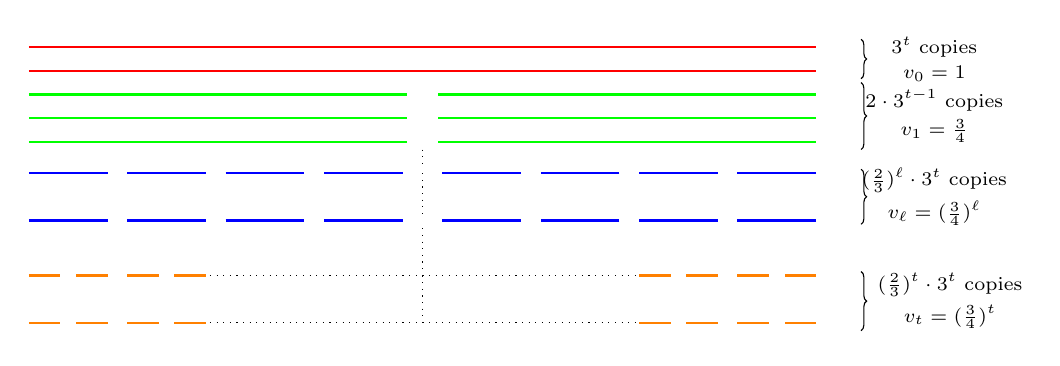
\begin{tikzpicture}
			\draw [red, thick] (-5,5) to (5,5);
			\draw [red, thick] (-5,4.7) to (5,4.7);
			
			\draw [decorate,decoration={brace,amplitude=2pt,raise=2pt},yshift=0pt]
			(5.5,5.1) -- (5.5,4.6) node [black,midway,xshift=1cm] {
				\shortstack{ \scriptsize $3^t$ copies \\ \scriptsize $v_0 = 1$}};
			
			\draw [green, thick] (-5,4.4) to (-0.2,4.4);
			\draw [green, thick] (0.2,4.4) to (5,4.4);
			
			\draw [green, thick] (-5,4.1) to (-0.2,4.1);
			\draw [green, thick] (0.2,4.1) to (5,4.1);			
			
			\draw [green, thick] (-5,3.8) to (-0.2,3.8);
			\draw [green, thick] (0.2,3.8) to (5,3.8);			
			
			\draw [decorate,decoration={brace,amplitude=2pt,raise=2pt},yshift=0pt]
			(5.5,4.55) -- (5.5,3.7) node [black,midway,xshift=1cm] {
			\shortstack{ \scriptsize $2 \cdot 3^{t-1}$ copies \\ \scriptsize $v_1 = \frac{3}{4}$}};			
		
			\draw[dotted]  (0, 3.7) -- (0, 3.45);
			
			\draw [blue, thick] (-5,3.4) to (-4,3.4);
			\draw [blue, thick] (-3.75,3.4) to (-2.75,3.4);			
			\draw [blue, thick] (-2.5,3.4) to (-1.5,3.4);			
			\draw [blue, thick] (-1.25,3.4) to (-0.25,3.4);									
			\draw [blue, thick] (5,3.4) to (4,3.4);
			\draw [blue, thick] (3.75,3.4) to (2.75,3.4);			
			\draw [blue, thick] (2.5,3.4) to (1.5,3.4);			
			\draw [blue, thick] (1.25,3.4) to (0.25,3.4);			
			
			\draw[dotted]  (0, 3.4) -- (0, 2.85);
			
			\draw [blue, thick] (-5,2.8) to (-4,2.8);
			\draw [blue, thick] (-3.75,2.8) to (-2.75,2.8);			
			\draw [blue, thick] (-2.5,2.8) to (-1.5,2.8);			
			\draw [blue, thick] (-1.25,2.8) to (-0.25,2.8);									
			\draw [blue, thick] (5,2.8) to (4,2.8);
			\draw [blue, thick] (3.75,2.8) to (2.75,2.8);			
			\draw [blue, thick] (2.5,2.8) to (1.5,2.8);			
			\draw [blue, thick] (1.25,2.8) to (0.25,2.8);
			
			\draw [decorate,decoration={brace,amplitude=2pt,raise=2pt},yshift=0pt]
			(5.5,3.45) -- (5.5,2.75) node [black,midway,xshift=1cm] {
				\shortstack{ \scriptsize $(\frac{2}{3})^\ell \cdot 3^{t}$ copies \\ \scriptsize $v_\ell = (\frac{3}{4})^{\ell}$}};			
			
			\draw[dotted]  (0, 2.7) -- (0, 2.1);
			
			\draw [orange, thick] (-5,2.1) to (-4.6,2.1);
			\draw [orange, thick] (-4.4,2.1) to (-4,2.1);
			\draw [orange, thick] (-3.75,2.1) to (-3.35,2.1);
			\draw [orange, thick] (-3.15,2.1) to (-2.75,2.1);			
			\draw[dotted] (-2.7, 2.1) to (2.7, 2.1)			;
			\draw [orange, thick] (5,2.1) to (4.6,2.1);
			\draw [orange, thick] (4.4,2.1) to (4,2.1);
			\draw [orange, thick] (3.75,2.1) to (3.35,2.1);
			\draw [orange, thick] (3.15,2.1) to (2.75,2.1);			
			
			
			\draw[dotted]  (0, 2.1) -- (0, 1.5);
			
			\draw [orange, thick] (-5,1.5) to (-4.6,1.5);
			\draw [orange, thick] (-4.4,1.5) to (-4,1.5);
			\draw [orange, thick] (-3.75,1.5) to (-3.35,1.5);
			\draw [orange, thick] (-3.15,1.5) to (-2.75,1.5);			
			\draw[dotted] (-2.7, 1.5) to (2.7, 1.5)			;
			\draw [orange, thick] (5,1.5) to (4.6,1.5);
			\draw [orange, thick] (4.4,1.5) to (4,1.5);
			\draw [orange, thick] (3.75,1.5) to (3.35,1.5);
			\draw [orange, thick] (3.15,1.5) to (2.75,1.5);			
			
			\draw [decorate,decoration={brace,amplitude=2pt,raise=2pt},yshift=0pt]
			(5.5,2.15) -- (5.5,1.4) node [black,midway,xshift=1.2cm] {
				\shortstack{ \scriptsize $(\frac{2}{3})^{t} \cdot 3^{t}$ copies \\ \scriptsize $v_{t} = (\frac{3}{4})^{t}$}};			
			
			
		\end{tikzpicture}
	}
	\caption{Laminar family construction for the lower bound of Lemma~\ref{lem:lb3}.}
	\label{fig:laminar}
\end{figure}

\begin{proof}

We construct a laminar family of sets arranged in binary tree fashion as follows: The root node is the set of all $n = 2^{t}$ items. At depth $\ell$, there are $2^\ell$ sets, each of size $\left( \frac{n}{2^{\ell}} \right)$ formed by partitioning each set at depth $\ell-1$ of size $\left( \frac{n}{2^{\ell - 1}} \right)$ into two. Further, each set $S$ at depth $\ell$ has valuation $v(S) = \left( \frac{3}{4} \right)^{\ell}$ and $c_\ell = \left( \frac{2}{3} \right)^{\ell} 3^t$ copies of itself. Figure~\ref{fig:laminar} shows the construction. Let $\mL$ denote the family of laminar sets in the construction. Although $v$ is only defined on $\mL$, it can be extended to any set $A\subseteq V$ by defining $v(A) = \min_{X \subseteq \mL} \sum_{S \in X} v(S)$ where $X$ is a set cover of $A$. Note that $v(A)$ is monotone and subadditive. We first prove that $v(A)$ is actually submodular.

Let us introduce some more notations. Let $\bA$ denote the minimum weighted set covering of a set $A$, i.e. $\bA = \argmin_{X \subseteq \mL} \sum_{S \in X} v(S)$  where $X$ is a set cover of $A$. We overload the valuation function $v$ to mean $v(\bA) = \sum_{S \in \bA} v(S)$ and define $A^{*} = \bigcup_{X \in \bA} X$ to be the set of items covered by some set in $X$. For any two sets $A, B \in 2^{[n]}$, it holds that $v(A) + v(B) = v(\bA) + v(\bB)$ by definition of valuation function. Observe that $A \cap B \subseteq A^{*} \cap B^{*}$ and by monotonicity, we have $v(A \cap B) \leq v(A^{*} \cap B^{*})$. Similarly, $v(A \cup B) \leq v(A^{*} \cup B^{*})$. Thus, to show submodularity, it suffices to verify that 
\begin{equation}\label{eqnsubmodular}
v(\bA) + v(\bB) \geq v(A^{*} \cup B^{*}) + v(A^{*} \cap B^{*}).
\end{equation}
Assume that the largest set in $\bA\cup \bB$ has size $2^u$. We verify (\ref{eqnsubmodular}) by applying induction to $u$.

\smallskip
\introparagraph{Base Case} If $u=0$, i.e. $\bA$ and $\bB$ only contain sets with size 1, let $L^{0}_1, \dots, L^{0}_{n} \in \mL$ denote all singleton sets. Define for each $i$ $A_i = A^* \cap L^{0}_i, B_i = B^* \cap L^{0}_i$. Then
\begin{eqnarray*}
	& &v(\bA) + v(\bB) \\
	&=& v(A_1) + \dots + v(A_n) +  v(B_1) + \dots + v(B_n) \\
	& = & v(A_1) + v(B_1) + \dots + v(A_n) + v(B_n) \\
	& = & v(A_1 \cap B_1) + \dots + v(A_n \cap B_n) + v(A_1 \cup B_1) + \dots + v(A_n \cup B_n) \\
	& = & v((A^* \cap B^*) \cap L^{0}_1) + \dots + v( (A^* \cap B^*) \cap L^{0}_n) +  v( (A^* \cup B^*) \cap L^{0}_1) + \dots + v( (A^* \cup B^*) \cap L^{0}_n) \\
	& \geq & v(A^{*} \cup B^{*}) + v(A^{*} \cap B^{*}).
\end{eqnarray*}
Here the first equality holds since $v(\bA)$ and $v(\bB)$ are defined only by sets with size 1.
The third equality holds since each $\bA_i$ and $\bB_i$ is either an empty set or singleton. The fourth equality holds by definition of $A_i$ and $B_i$. The fifth inequality holds by subadditivity of $v$.

\smallskip
\introparagraph{Inductive Case} Assume that $v(\bA) + v(\bB) \geq v(A^{*} \cup B^{*}) + v(A^{*} \cap B^{*})$ holds if all sets in $\bA\cup \bB$ have size at most $2^{u-1}$. Consider all sets of size $2^u$: $L^{u}_1, \dots, L^{u}_{n/2^u} \in \mL$ and define for every $i$ $A_i = A^* \cap L^{u}_i, B_i = B^* \cap L^{u}_i$. Using the same argument as in the base case, we have 

\begin{eqnarray*}
& &v(\bA) + v(\bB)\\
& = &v(A_1) + \dots + v(A_{n/2^{u}}) +  v(B_1) + \dots + v(B_{n/2^{u}})\\
& =  & v(A_1) + v(B_1) + \dots + v(A_{n/2^{u}}) + v(B_{n/2^{u}}) \\
& \geq & v(A_1 \cap B_1) + \dots + v(A_{n/2^{u}} \cap B_{n/2^{u}}) + v(A_1 \cup B_1) + \dots + v(A_{n/2^{u}} \cup B_{n/2^{u}}) \\
& = & v( (A^* \cap B^*) \cap L^{u}_1) + \dots + v( (A^* \cap B^*) \cap L^{u}_{n/2^{u}}) +  v( (A^* \cup B^*) \cap L^{u}_1) + \dots + v( (A^* \cup B^*) \cap L^{u}_{n/2^{u}}) \\
&\geq &v(A^{*} \cup B^{*}) + v(A^{*} \cap B^{*}).
\end{eqnarray*}

Here the third inequality is where we invoke the inductive hypothesis: if $v(A_i)=v(L_i^u)$ or $v(B_i)=v(L_i^u)$, then $v(A_i)+v(B_i)=v(A_i\cup B_i)+v(A_i\cap B_i)$. Otherwise, $v(A_i)$ and $v(B_i)$ are both defined by sets with size at most $2^{u-1}$, by inductive hypothesis $v(A_i)+v(B_i)\geq v(A_i\cup B_i)+v(A_i\cap B_i)$. Thus (\ref{eqnsubmodular}) always holds, which means $v$ is indeed a submodular function.

If we price every bundle at its value, the revenue extracted is maximized. For each level $\ell$, there are $2^{\ell}$ sets and $(2/3)^{\ell} \cdot 3^{t}$ copies of each set. Thus, the total revenue from all $t+1$ levels is
\begin{align*}
	\textsf{OPT} = \sum_{\ell = 0}^{t} v_\ell c_\ell 2^\ell = (t+1)\left( \frac{3}{4} \right)^{\ell}  \cdot \left( \frac{4}{3} \right)^{\ell} \cdot  3^{t} = (t+1) \cdot 3^{t}.
\end{align*}

%However, it remains to be shown that the third inequality is true, i.e. $v(\bA_i) + v(\bB_i) \geq v(\bA_i \cup \bB_i) + v(\bA_i \cap \bB_i)$. If either $\bA_i = L^{u}_i$ or $\bB_i = L^{u}_i$, then the inequality (equality in this case) holds.

%Otherwise, if each $\bA_i$ and $\bB_i$ is empty, it means that $\bA_i$ and $\bB_i$ are covered by sets with height $< u$. Define $\bA'_i = \bA_i \cap L^{u-1}_i, \bB'_i = \bB_i \cap L^{u-1}_i$. By the inductive hypothesis, it holds that $v(\bA'_i) + v(\bB'_i) \geq v(\bA'_i \cup \bB'_i) + v(\bA'_i \cap \bB'_i)$ and thus,

%\begin{align*}
%	v(\bA_i) + v(\bB_i) & = v(\bA'_1) + \dots + v(\bA'_{n/2^{u-1}}) +  v(\bB'_1) + \dots + v(\bB'_{n/2^{u-1}}) \displaybreak[0]\\
%	& = v(\bA'_1) + v(\bB'_1) + \dots + v(\bA'_{n/2^{u-1}}) + v(\bB'_{n/2^{u-1}}) \displaybreak[0] \\
%	& \geq v(\bA'_1 \cap \bB'_1) + \dots + v(\bA'_{n/2^{u-1}} \cap \bB'_{n/2^{u-1}}) + v(\bA'_1 \cup \bB'_1) + \dots + v(\bA'_{n/2^{u-1}} \cup \bB'_{n/2^{u-1}}) \displaybreak[0]\\
%	& = v( (\bA_i \cap \bB_i) \cap L^{u-1}_1) + \dots + v( (\bA_i \cap \bB_i) \cap L^{u-1}_{n/2^{u-1}}) +  v( (\bA_i \cup \bB_i) \cap L^{u-1}_1) + \dots + v( (\bA_i \cup \bB_i) \cap L^{u-1}_{n/2^{u-1}}) \displaybreak[0]\\
%	& \geq v(\bA_i \cup \bB_i) + v(\bA_i \cap \bB_i)	
%\end{align*}

Next, we will show that no uniform bundle pricing or item pricing can extract revenue more than $O(3^{t})$.

For optimal bundle pricing, the first observation is that we need to consider only bundle prices of the form $\left( \frac{3}{4} \right)^{k}$, i.e. the value of some set in the laminar system. Let the bundle price chosen be $\left(\frac{3}{4} \right)^{k}$, then we can sell all edges at depth $\leq k$. The revenue collected by such bundle pricing is 
\begin{equation*}
\textsf{OPT}_B = \sum_{i \leq k} \left( \frac{3}{4} \right)^{k} \cdot \left( \frac{2}{3} \right)^{i} \cdot 3^{t} \cdot 2^{i} 
 = \left( \frac{3}{4} \right)^{k} \cdot 3^{t} \sum_{i \leq k} \left( \frac{4}{3} \right)^{i} \displaybreak[0]\\
 \leq \left( \frac{3}{4} \right)^{k} \cdot 3^{t+1} \cdot \left( \frac{4}{3} \right)^{k} = O(3^{t}).
\end{equation*}

For optimal item pricing, let $k$ be the smallest depth for any set sold by an optimal item pricing solution. By symmetry we can assume that all sets with depth $k$ are sold. Then the sum of prices of all items is upper bounded by $\sum_{i}p_i\leq (\frac{3}{4})^{k}\cdot 2^k=(\frac{3}{2})^k$, since there are $2^k$ distinct sets with depth $k$. Thus the revenue of such item pricing is contributed by sets with depth at least $k$, and can be upper bounded by
\begin{equation*}
\textsf{OPT}_{IP}\leq\sum_{\ell\geq k}\left(\frac{3}{2}\right)^k\cdot c_\ell=\left( \frac{3}{2} \right)^{k} \cdot   3^{t} \sum_{\ell \geq k} \left( \frac{2}{3} \right)^{\ell}
\leq \left( \frac{3}{2} \right)^{k} \cdot  3^{t+1} \cdot  \left( \frac{2}{3} \right)^{k} 
=O(3^{t})
\end{equation*}
since each set in level $\ell$ has $c_\ell$ copies.

In conclusion the revenue gap between $\textsf{OPT}$ and $\max(\textsf{OPT}_B,\textsf{OPT}_{IP})$ is $\Omega(t)$. Note that $m = \sum_{k = 0}^{t} 3^{t} \cdot  2^{k} \cdot  \left( \frac{2}{3} \right)^{k} \leq 3^{t} \cdot  \left( \frac{4}{3} \right)^{t+1} = O(4^{t})$ and thus, the revenue gap is $\Omega(\log m)$. 


\end{proof}


\section{Skewed Workload}
\label{sec:skewed:workload}

Table~\ref{table:worldqueries} lists the queries used for the skewed workload on $\texttt{\bfseries world}$ dataset. To increase the number of queries to $986$, we add a new query for every country (in the domain of the attribute) by changing the predicate in $Q_{17}, Q_{27}, Q_{31}$, for every continent in $Q_1, Q_{12}$ and for every language in $Q_{29}, Q_{30}$.

\begin{table}
	\begin{tabular}{l|L{12cm}}
		\toprule
		& \textbf{Query}  \\
		\midrule
		
		$Q_1$ & \texttt{
			select count(Name) from Country where Continent = `Asia'
		} \\ \hdashline 
		
		$Q_2$ & \texttt{
			select count(distinct Continent) from Country
		} \\ \hdashline
		
		$Q_3$ & \texttt{
			select avg(Population) from Country 
		} \\ \hdashline
		
		$Q_4$ & \texttt{
			select max(Population) from Country
		} \\ \hdashline
		
		$Q_5$ & \texttt{
			select min(LifeExpectancy) from Country
		} \\ \hdashline
		
		$Q_6$ & \texttt{
			select count(Name) from Country where Name like `A%' 
		} \\ \hdashline
		
		$Q_7$ & \texttt{
			select Region, max(SurfaceArea) from Country group by Region 
		} \\ \hdashline
		
		$Q_8$ & \texttt{
			select Continent, max(Population) from Country group by Continent
		} \\ \hdashline
		
		$Q_9$ & \texttt{
			select Continent, count(Code) from Country group by Continent
		}\\
		
		
		$Q_{10}$ & \texttt{
			select * from Country
		} \\ \hdashline
		
		$Q_{11}	$ & \texttt{
			select Name from Country where Name like 'A\%'
		} \\ \hdashline
		
		$Q_{12}$ & \texttt{
			select * from Country where Continent='Europe' and Population > 5000000 
		} \\ \hdashline
		
		$Q_{13}$ & \texttt{
			select * from Country where Region='Caribbean' 
		} \\ \hdashline
		
		$Q_{14}$ & \texttt{
			select Name from Country where Region='Caribbean'
		}\\
		
		$Q_{15}$ & \texttt{
			select Name from Country where Population between 10000000 and 20000000
		} \\ \hdashline
		
		$Q_{16}$ & \texttt{
			select * from Country where Continent='Europe' limit 2
		} \\ \hdashline
		
		$Q_{17}$ & \texttt{
			select Population from Country where Code = USA'
		} \\ \hdashline
		
		$Q_{18}$ & \texttt{
			select GovernmentForm from Country
		} \\ \hdashline
		
		$Q_{19}$ & \texttt{
			select distinct GovernmentForm from Country
		} \\ \hdashline
		
		$Q_{20}$ & \texttt{
			select * from City where Population >= 1000000 and CountryCode = 'USA' 
		} \\ \hdashline
		
		$Q_{21}$ & \texttt{
			select distinct Language from CountryLanguage where CountryCode='USA'
		} \\ \hdashline
		
		$Q_{22}$ & \texttt{
			select * from CountryLanguage where IsOfficial = 'T'
			'} \\ \hdashline
		
		$Q_{23}$ & \texttt{
			select Language, count(CountryCode) from CountryLanguage group by Language
		} \\ \hdashline
		
		$Q_{24}$ & \texttt{
			select count(Language) from CountryLanguage where CountryCode = 'USA'
		} \\ \hdashline
		
		$Q_{25}$ & \texttt{
			select CountryCode, sum(Population) from City group by CountryCode 
		} \\ \hdashline
		
		$Q_{26}$ & \texttt{
			select CountryCode, count(ID) from City group by CountryCode 
		} \\ \hdashline
		
		$Q_{27}$ & \texttt{
			select * from City where CountryCode = 'GRC'
		} \\ \hdashline
		
		$Q_{28}$ & \texttt{
			select distinct 1 from City where CountryCode = 'USA' and Population > 10000000
		} \\ \hdashline
		
		$Q_{29}$ & \texttt{
			select Name from Country , CountryLanguage where Code = CountryCode and Language = 'Greek'
		} \\ \hdashline
		
		$Q_{30}$ & \texttt{
			select C.Name from Country C, CountryLanguage L where C.Code = L.CountryCode and L.Language = 'English' and L.Percentage >= 50
		} \\ \hdashline
		
		$Q_{31}$ & \texttt{
			select T.district from Country C, City T where C.code = 'USA' and C.capital = T.id
		} \\ \hdashline
		
		$Q_{32}$ & \texttt{
			select * from Country C, CountryLanguage L where C.Code = L.CountryCode and L.Language = 'Spanish'
		} \\ \hdashline
		
		$Q_{33}$ & \texttt{
			select Name, Language from Country , CountryLanguage where Code = CountryCode 
		} \\ \hdashline
		
		$Q_{34}$ & \texttt{
			select * from Country , CountryLanguage where Code = CountryCode
		} \\ \hdashline
		
	\end{tabular}
	\vspace{2mm}
	\caption{Queries used for \texttt{world} database}
	\label{table:worldqueries}
\end{table}




\end{document}

